\documentclass[journal]{IEEEtran}
\usepackage{cite}
\usepackage{amsmath,amssymb,amsfonts,amsthm}
\usepackage{algorithm}
\usepackage{algpseudocode}
\usepackage{graphicx}
\usepackage{booktabs}
\usepackage{multirow}
\usepackage{xcolor}
\usepackage[hidelinks]{hyperref}
\usepackage{microtype}
\graphicspath{{../figures/}{../../docs/figures/}}
\newtheorem{proposition}{Proposition}
\newtheorem{theorem}{Theorem}
\newtheorem{corollary}{Corollary}
\newcommand{\LS}{\mathbf{L}}
\newcommand{\cf}{\mathrm{CF}}
\hyphenation{Fed-CAST micro-cluster micro-clusters Kafka}

\begin{document}

\title{Communicating by Value: Budget-Aware Federated\\ Stream Clustering over Apache Kafka for\\ Evolving Non-IID Edge Streams}

\author{Author~One,~\IEEEmembership{Student Member,~IEEE,}
        Author~Two,~\IEEEmembership{Student Member,~IEEE,}
        and~Author~Three,~\IEEEmembership{Member,~IEEE}%
\thanks{The authors are with the Department of Computer Science, University Name, City, Country (e-mail: author@university.edu).}%
\thanks{Code, configurations, raw results and scripts that regenerate every figure and table are publicly available in the project repository.}}

\markboth{Preprint}{One \MakeLowercase{\textit{et al.}}: Communicating by Value: Budget-Aware Federated Stream Clustering}

\maketitle

\begin{abstract}
Edge devices produce unlabeled, non-IID data streams over constrained links, and operators need a continuously updated global clustering without collecting raw data. Every device must repeatedly decide whether an update is worth its network cost and which part of its local model to send. Existing systems answer with a schedule (periodic or one-shot federated clustering) or, as in communication-efficient federated learning, by the magnitude of the change. We show that the right quantity is the \emph{value} of an update. When a coordinator computes a cluster centre from stale summaries, its k-means cost exceeds the optimum by exactly $\|\Delta L_j-\Delta N_j\hat c_j\|^2/N_j$, a closed form that every device can evaluate for its own micro-clusters from the broadcast model. Growth of a cluster in place is worth nothing, whereas the first points of an emerging cluster are worth a lot. We build FedCAST on this criterion: value-greedy selection of cluster-feature deltas, a scale-free dual-ascent threshold with a hard token-bucket budget and use-it-or-lose-it sends, 8-bit deltas with error feedback, and a staleness-robust approximation guarantee $J\le\gamma\,\mathrm{OPT}+(1+\gamma)U$. FedCAST runs on Apache Kafka, whose per-key ordering, idempotent producers and log-compacted changelog provide exactly-once state and crash recovery, in under 1\,GB of RAM. Over 3{,}800 seeded runs on eight datasets, including three naturally drifting real streams, value-based communication beats the strongest federated-learning compressor (top-$k$ magnitude with error feedback, equally quantized) in 72\,\% of 200 paired non-stationary comparisons ($p=4\times10^{-11}$) and in 75\,\% on naturally drifting real data ($p=2\times10^{-6}$), while tying on static streams. Both far outperform periodic synchronization and k-FED. A multi-container deployment with kernel-enforced bandwidth caps confirms the gains end to end.
\end{abstract}

\begin{IEEEkeywords}
Federated clustering, data streams, concept drift, communication efficiency, non-IID data, edge computing, Apache Kafka.
\end{IEEEkeywords}

\section{Introduction}
\IEEEPARstart{N}{etwork} probes, industrial gateways, sensor motes and vehicles continuously produce unlabeled data streams at the edge. Operators want one continuously updated \emph{global} view of the structure in these streams, such as the traffic profiles present in a network right now or the operating regimes of a sensor field. Three constraints stand in the way. Raw data often cannot leave the device, for legal, privacy or volume reasons. The data are \emph{non-IID}: each device sees a different slice of the global distribution, and some patterns appear at a single device only. And links are constrained: metered cellular uplinks, lossy wireless and intermittent connectivity make every byte costly.

Stream clustering handles the first constraint with compact, additive micro-cluster summaries~\cite{zhang1996birch,aggarwal2003clustream,cao2006denstream}. Distributed variants ship these summaries to a coordinator~\cite{cormode2007divide,gama2011dgclust,tran2013communication}, and federated clustering copes with heterogeneity on static data~\cite{dennis2021kfed,zhang2025afcl}. Every edge node, however, faces a question at every instant that none of these works answers in a principled way: \emph{is sending an update now worth its network cost, and if so, which part of the model should be sent?} Schedules (periodic updates, one-shot federated clustering) waste bytes when nothing changes and leave the coordinator stale exactly when the data drift. Communication-efficient federated learning ranks updates by their \emph{magnitude}, e.g.\ top-$k$ sparsification with error feedback~\cite{aji2017sparse,stich2018sparsified,karimireddy2019ef}. As we show, magnitude is the wrong currency for clustering: large changes are often worthless (a cluster growing in place), and small ones can be critical (the first points of a new cluster).

\textbf{Key insight.} With the assignment of summaries to centres fixed, the extra k-means cost that staleness causes at the coordinator has an \emph{exact closed form}: for a centre $\hat c_j$ computed from stale summaries, the cost exceeds its optimum by $\|\Delta L_j-\Delta N_j\hat c_j\|^2/N_j$, where $\Delta L_j,\Delta N_j$ are the unsent changes of the linear sum and mass of cluster~$j$ (Proposition~\ref{prop:exact}). Each device knows its own contribution to these quantities and receives $\hat c_j,N_j$ with the global model, so it can compute the exact \emph{value} of sending each of its micro-clusters.

\textbf{Contributions.}
\begin{enumerate}
\item \emph{Value of an update.} The closed-form value above, its marginal form for greedy selection, and the observation that it is zero for in-place growth and large for emerging mass.
\item \emph{FedCAST}, a budget-aware federated stream clustering system built on this value: value-greedy cluster-feature (CF) deltas with a magnitude tie-break, a scale-free exponentiated dual-ascent threshold, a hard token-bucket budget with use-it-or-lose-it sends, and 8-bit deltas with error feedback.
\item \emph{Guarantees}: a staleness-robust approximation bound $J(S;\hat C)\le\gamma\,\mathrm{OPT}(S)+(1+\gamma)U$ with a model-free, locally computable staleness $U$ (Theorem~\ref{thm:robust}), and a hard and long-run budget guarantee (Proposition~\ref{prop:budget}).
\item \emph{A Kafka-native system}: per-key ordering, idempotent producers with sequence numbers, and a log-compacted changelog give exactly-once state and crash recovery without resends, in under 1\,GB of RAM.
\item \emph{A rigorous evaluation}: 3{,}800+ seeded runs on eight datasets (static, drifting, evolving, and three \emph{naturally} drifting real streams, one of them naturally partitioned by device), paired statistical tests against an equally quantized top-$k$ compressor, real-broker fault injection, and a multi-container deployment with kernel bandwidth caps. We also report the ideas that did \emph{not} work.
\end{enumerate}

\section{Related Work}\label{sec:related}
\textit{Stream clustering.} CluStream~\cite{aggarwal2003clustream} introduced online micro-clusters with offline macro-clustering, building on BIRCH cluster features~\cite{zhang1996birch}. DenStream~\cite{cao2006denstream} added decay and density-based macro-clustering, and DBSTREAM~\cite{hahsler2016dbstream} a shared-density graph; see~\cite{zubaroglu2021review,gama2014survey} for surveys of stream clustering and concept drift.

\textit{Distributed stream clustering.} Cormode et al.~\cite{cormode2007divide} maintain a continuous k-center clustering over distributed streams. DGClust~\cite{gama2011dgclust} reports grid-cell state changes, and Tran and Sattler~\cite{tran2013communication} ship micro-clusters to a coordinator. Coresets~\cite{balcan2013distributed} give strong guarantees on static data. These methods send on fixed rules and have neither a byte budget nor a notion of the value of an update.

\textit{Federated clustering.} k-FED~\cite{dennis2021kfed} performs one-shot federated k-means and shows that heterogeneity can help. FFCM~\cite{stallmann2022ffcm} and AFCL~\cite{zhang2025afcl} extend federated clustering to fuzzy memberships and to asynchrony with unknown $k$. All assume static local data. FedCluLearn~\cite{angelova2025fedclulearn} and federated anomaly detection on streams~\cite{silva2022federated,li2025dfas} target supervised or anomaly-detection objectives.

\textit{Communication-efficient learning.} Federated learning~\cite{mcmahan2017fedavg,kairouz2021advances} reduces traffic by sparsification (top-$k$)~\cite{aji2017sparse,lin2018dgc,sattler2020stc}, quantization~\cite{alistarh2017qsgd} and error feedback~\cite{stich2018sparsified,karimireddy2019ef}, and by event-triggered communication~\cite{ghosh2021eventgrad,zehtabi2022event}. These methods rank coordinates by magnitude. We use sparsification, quantization and error feedback as building blocks, but rank by the exact effect on the clustering objective, and we compare against magnitude ranking under identical quantization.

\textit{Kafka for machine learning.} Kafka-ML~\cite{martin2022kafkaml,carnerero2024kafkaml} uses Kafka to train neural networks federatedly. We use Kafka's semantics as part of the correctness and recovery argument, following the changelog pattern of stream processors~\cite{kreps2011kafka,carbone2017flinkstate}.

\section{Problem Formulation}\label{sec:problem}
There are $m$ edge nodes. Node $i$ receives points $x\in\mathbb{R}^d$ from a time-varying, non-IID distribution $P_i(t)$, and the global distribution is the mixture $P(t)$. Node $i$ summarizes its stream by at most $q$ micro-clusters with time-decayed cluster features~\cite{zhang1996birch,cao2006denstream}
\begin{equation}
\begin{split}
\cf&=(n,\ \LS,\ SS,\ \tau),\\
n&=\textstyle\sum w_x,\quad \LS=\sum w_x x,\quad SS=\sum w_x\|x\|^2,
\end{split}
\end{equation}
with weights $w_x=2^{-(t-t_x)/H}$ and last update $\tau$. Decay scales all three sums by one factor, so centroids and radii are decay-invariant, and a copy of a CF plus its $\tau$ determines its decayed value at any time. The k-means cost of the points summarized by a CF at centre $c$ is
\begin{equation}\label{eq:cost}
J(\cf,c)=SS-2\LS^{\!\top}c+n\|c\|^2 .
\end{equation}
The coordinator stores the last CFs received from each node, $\hat S_i$, and publishes global centres $C=\{c_j\}$ with masses $N_j$. Node $i$ may send at most $B_i$ bytes per window $W$ over a link with price $p_i\ge1$. The goal is to keep $J(C(t);P(t))$ close to a centralized learner with all raw data, subject to the budgets.

\section{FedCAST}\label{sec:method}

\begin{figure*}[t]
\centering
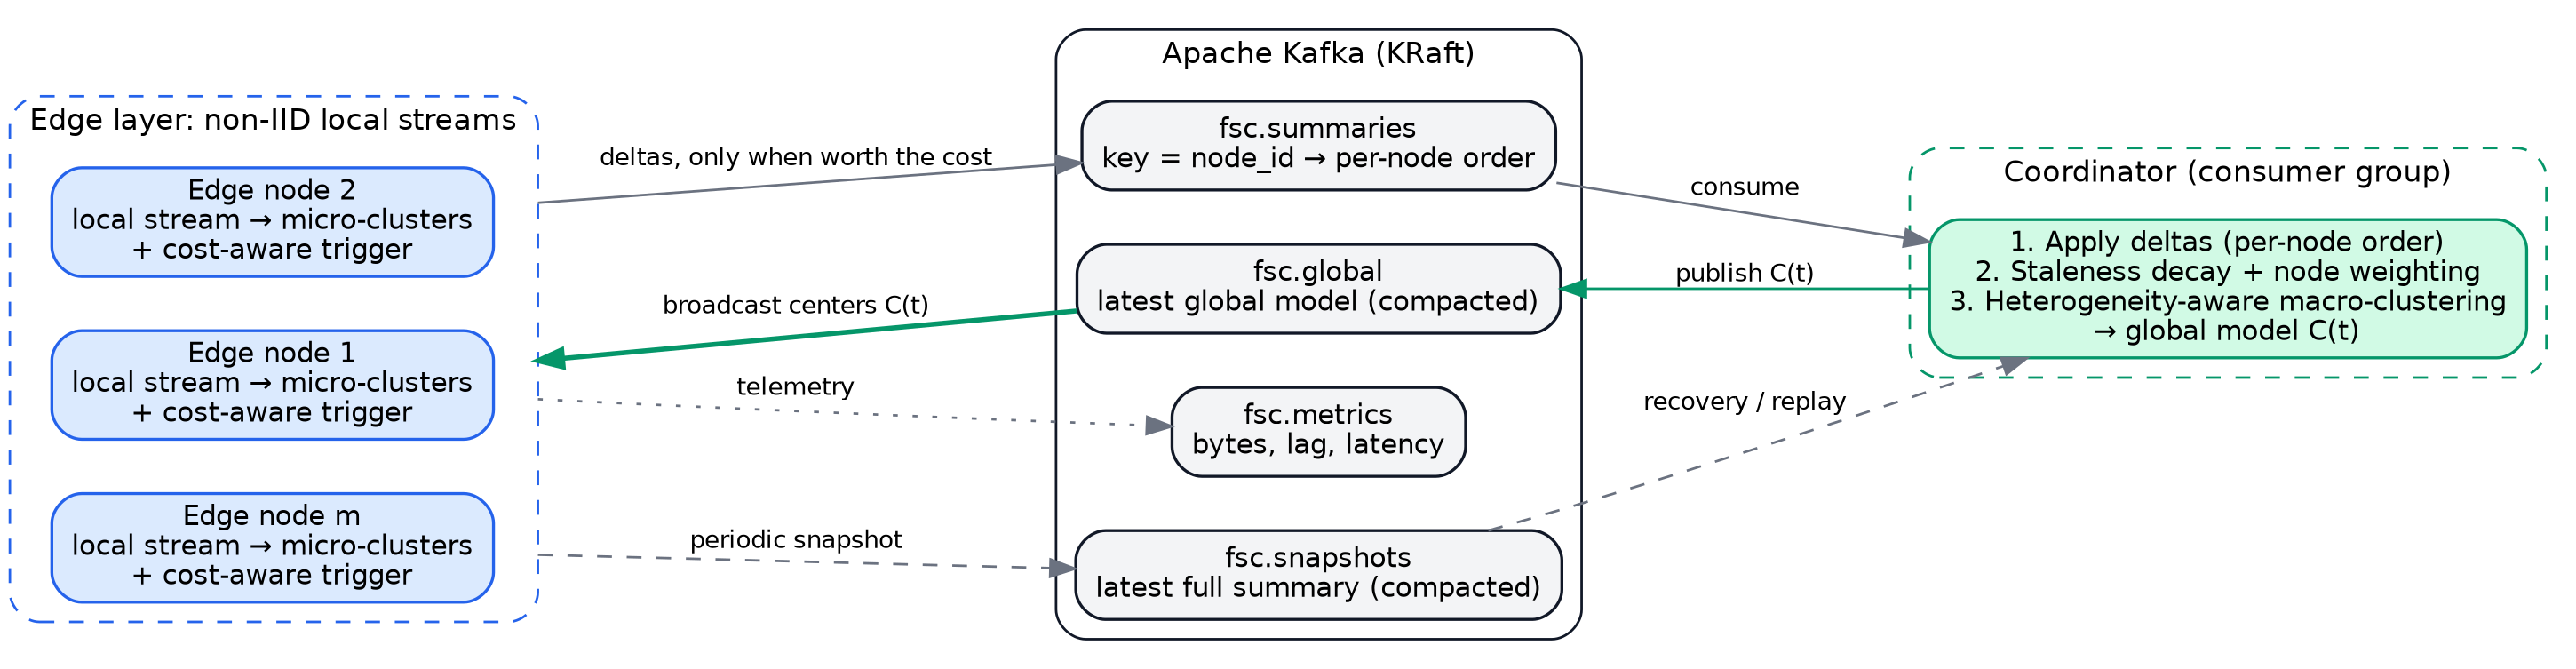
\includegraphics[width=0.95\textwidth]{architecture.png}
\caption{FedCAST over Apache Kafka. Edge nodes publish value-ranked, 8-bit CF deltas only when they are worth their byte cost. The coordinator applies them exactly once in per-node order, checkpoints to a compacted changelog, and broadcasts the global model (centres and masses) on a compacted topic, from which the edges compute the value of their updates.}\label{fig:arch}
\end{figure*}

\subsection{Local Summarization}
Each node runs a CluStream-style update~\cite{aggarwal2003clustream} with DenStream-style decay~\cite{cao2006denstream}. A point joins the nearest micro-cluster if it lies within twice its RMS radius (with a floor); otherwise it opens a new one. When all $q$ slots are full, a stale micro-cluster is pruned or the two closest are merged, using an exact nearest-neighbour cache updated in $O(qd)$. The node keeps an exact copy of the CFs it has sent, which is precisely the coordinator's view, because both sides apply the same deterministic decay.

\subsection{The Value of an Update}
\begin{proposition}[Exact staleness excess]\label{prop:exact}
Fix the assignment of CFs to global clusters. Let the coordinator's centre of cluster $j$ be $\hat c_j=\hat L_j/\hat N_j$, computed from the stale summaries, and let the true aggregates be $L_j=\hat L_j+\Delta L_j$ and $N_j=\hat N_j+\Delta N_j$. Then
\begin{equation}\label{eq:excess}
J_j(\hat c_j)-\min_c J_j(c)=\frac{\|\Delta L_j-\Delta N_j\,\hat c_j\|^2}{N_j}.
\end{equation}
\end{proposition}
\begin{IEEEproof}
By~\eqref{eq:cost}, $J_j(c)=SS_j-2L_j^{\!\top}c+N_j\|c\|^2$ is minimized at $c^*=L_j/N_j$, and $J_j(\hat c)-J_j(c^*)=N_j\|\hat c-c^*\|^2=\|N_j\hat c-L_j\|^2/N_j$. Since $\hat N_j\hat c_j=\hat L_j$, we have $N_j\hat c_j-L_j=\Delta N_j\hat c_j-\Delta L_j$.
\end{IEEEproof}

\begin{corollary}\label{cor:inplace}
Growth of a cluster in place ($\Delta L_j=\Delta N_j\hat c_j$) has zero value, however large $\Delta N_j$ is. Mass $\Delta N$ arriving at distance $\delta$ from $\hat c_j$ has value $\Delta N^2\delta^2/N_j$: quadratic in distance and inversely proportional to the size of the global cluster.
\end{corollary}

Magnitude-based compressors~\cite{aji2017sparse,stich2018sparsified} rank updates by $\|(\Delta n,\Delta\LS,\Delta SS)\|$. They therefore spend bytes on the first kind of change and may delay the second, which is exactly what matters under concept evolution.

\textit{Marginal value.} Node $i$ assigns each dirty micro-cluster to its nearest broadcast centre and accumulates its own residual $r_j=\sum(\Delta\LS_{\mathrm{id}}-\Delta n_{\mathrm{id}}\hat c_j)$ over all unsent changes, including deletions and micro-clusters that changed cluster. Sending micro-cluster \textit{id} removes its contribution $u_{\mathrm{id}}$ from $r_j$ and reduces the excess by
\begin{equation}\label{eq:marginal}
v_{\mathrm{id}}=\big(2\,u_{\mathrm{id}}^{\!\top}r_j-\|u_{\mathrm{id}}\|^2\big)/N_j ,
\end{equation}
which is exact for the node's own contribution (other nodes' residuals are unknown to it and enter only through cross terms). Micro-clusters are ranked by $v_{\mathrm{id}}$. Change magnitude, normalized and weighted by $\epsilon=0.1$, breaks ties among zero-value refinements: \emph{value first, information second}.

\subsection{Budgeted Sending}\label{sec:policy}
Once per tick, a node selects the smallest top-ranked set of micro-clusters covering a fraction $\gamma=0.9$ of its total score. Together with pending deletions, this set yields a payload of $b$ bytes with covered score $D$. The node sends if
\begin{equation}\label{eq:trigger}
D\ \ge\ \lambda_i\,p_i\,b \quad\text{or the token bucket is about to overflow,}
\end{equation}
provided the bucket (rate $B_i/W$, capacity $\kappa_i$) holds $b$ tokens. Tokens above capacity are lost, so a send when the bucket is nearly full has no opportunity cost (\emph{use-it-or-lose-it}). This prevents the node from under-spending once all remaining changes have near-zero value. Once per window, the threshold is updated by exponentiated dual ascent,
\begin{equation}\label{eq:dual}
\lambda_i\leftarrow\lambda_i\exp\!\big(\eta\ \mathrm{clip}_{[-1,2]}((\text{spent}_i-B_i)/B_i)\big),
\end{equation}
which is scale-free: the same $\eta=0.5$ works on every dataset. The price $p_i$ is an exponentially weighted estimate of retransmission overhead and delivery latency, obtained from producer delivery reports.

\begin{proposition}[Budget]\label{prop:budget}
(i) Over any interval of length $T$, node $i$ sends at most $\kappa_i+B_iT/W$ bytes. (ii) Without overflow sends, if $D\le D_{\max}$ and $b\ge b_{\min}$, the average relative overspend after $n$ windows is at most $\log(\lambda^\dagger e^{2\eta}/\lambda_0)/(\eta n)$ with $\lambda^\dagger=D_{\max}/b_{\min}$.
\end{proposition}
\begin{IEEEproof}
(i) Every send, including an overflow send, consumes its size from a bucket that starts at $\kappa_i$, refills at rate $B_i/W$, and never goes negative. (ii) Let $\theta=\log\lambda$. Telescoping~\eqref{eq:dual} gives $\sum_w g_w=(\theta_{n+1}-\theta_1)/\eta$. If $\lambda>\lambda^\dagger$, no send satisfies~\eqref{eq:trigger}, so $g_w=-1$. Hence $\theta$ never exceeds $\max(\theta_1,\log\lambda^\dagger)+2\eta$.
\end{IEEEproof}

\subsection{8-bit Deltas with Error Feedback}
A delta record carries an identifier, the count (float32), the variance (float16), a time offset (float32) and the centroid quantized to 8 bits per dimension relative to the message's own range (two float16 values per dimension). This is $14+d$ bytes per record instead of $24+4d$. The node stores the \emph{dequantized} record as its copy of the coordinator's view. Quantization error therefore shows up as ordinary staleness and is corrected by later sends (error feedback~\cite{karimireddy2019ef}), and the coordinator's state always equals the node's record of it.

\subsection{Aggregation}
The coordinator applies each delta exactly once (sequence numbers per node), decays all CFs to the current time so that silent nodes fade out, and runs weighted k-means over CF centroids. It warm-starts from the previous model and adds swap local search~\cite{kanungo2004local} and a k-means++ restart~\cite{arthur2007kmeanspp}. Warm starts keep cluster identities stable, and swaps prevent a cluster that appears at a single node from being absorbed by a warm-started neighbour. The coordinator broadcasts centres, radii and masses $N_j$.

\begin{algorithm}[t]
\caption{FedCAST edge node $i$ (one tick)}\label{alg:edge}
\small
\begin{algorithmic}[1]
\State ingest points into the decayed CF micro-clusters
\State refill token bucket; if no global model yet, send a bootstrap summary
\State for dirty micro-clusters: residuals $r_j$ and values $v_{\mathrm{id}}$ (Eq.~\ref{eq:marginal})
\State score $\gets v/\sum v+\epsilon\cdot\text{magnitude}/\sum\text{magnitude}$
\State $P\gets$ top-scored prefix covering $\gamma$ of the score; $b\gets$ bytes of $P$ (8-bit)
\If{($D\ge\lambda p b$ \textbf{or} bucket nearly full) \textbf{and} tokens $\ge b$}
  \State produce delta to \texttt{fsc.summaries}, key \texttt{node-}$i$; store dequantized copy
\EndIf
\State on \texttt{fsc.global}: update $\hat c_j,N_j$; at window end: update $\lambda$ (Eq.~\ref{eq:dual})
\end{algorithmic}
\end{algorithm}

\subsection{A Staleness-Robust Approximation Guarantee}
Proposition~\ref{prop:exact} is exact but holds for fixed assignments. The following model-free bound holds for \emph{any} aggregation algorithm.

\begin{theorem}[Staleness-robust approximation]\label{thm:robust}
Let every centre satisfy $\|c\|\le R$, and let
\[
U=\sum_i\sum_{\mathrm{id}}\big(|\Delta SS_{\mathrm{id}}|+2R\|\Delta\LS_{\mathrm{id}}\|+R^2|\Delta n_{\mathrm{id}}|\big)
\]
be the model-free staleness of all nodes (current versus coordinator copies). If the coordinator computes a $\gamma$-approximate k-means solution $\hat C$ on the stale summaries $\hat S$, then on the current summaries $S$,
\begin{equation}
J(S;\hat C)\ \le\ \gamma\,\mathrm{OPT}(S)+(1+\gamma)\,U .
\end{equation}
\end{theorem}
\begin{IEEEproof}
For $\|c\|\le R$, by~\eqref{eq:cost}, $|J(\cf,c)-J(\widehat{\cf},c)|=|\Delta SS-2\Delta\LS^{\!\top}c+\Delta n\|c\|^2|\le|\Delta SS|+2R\|\Delta\LS\|+R^2|\Delta n|$. Since $|\min_c a_c-\min_c b_c|\le\max_c|a_c-b_c|$, summing over micro-clusters gives $|J(S;C)-J(\hat S;C)|\le U$ for every $C$ in the $R$-ball. Optimal centres are convex combinations of data points and lie in the ball. Therefore $J(S;\hat C)\le J(\hat S;\hat C)+U\le\gamma\,\mathrm{OPT}(\hat S)+U\le\gamma(\mathrm{OPT}(S)+U)+U$.
\end{IEEEproof}

With 8-bit deltas, $\hat S$ is the dequantized view, so $U$ also covers quantization error. Both the exactness of~\eqref{eq:excess} and the bound of Theorem~\ref{thm:robust} are checked numerically in the test suite.

\textit{Complexity.} Per point: $O(qd)$. Per tick and node: $O(|\mathrm{dirty}|\,kd)$. Per aggregation: $O(I\,mq\,kd)$ over at most $mq$ micro-clusters, never over raw points.

\section{System Design on Apache Kafka}\label{sec:system}
Four Kafka semantics are part of FedCAST's correctness argument. \emph{Per-partition order}, with node identifier as key, lets a delta assume its predecessor. \emph{Idempotent producers} plus per-node sequence numbers make retries on lossy links harmless, and replays after a crash are ignored. The \emph{replayable log} with committed offsets means nodes never resend after a coordinator crash. \emph{Log compaction} keeps one changelog record per node in \texttt{fsc.snapshots} (server-side CFs with the applied sequence number and offsets as headers) and the latest model in \texttt{fsc.global}. On restart, the coordinator restores the compacted changelog and replays \texttt{fsc.summaries} from the checkpointed offsets, the state-store pattern of stream processors~\cite{carbone2017flinkstate}. Messages use a fixed binary layout whose size is known before encoding, as~\eqref{eq:trigger} requires. The broker runs in KRaft mode with a 256\,MB heap. The same node, policy, codec and coordinator classes run both against a real broker and inside a deterministic discrete-event simulator. The simulator emulates per-node links (delay, jitter, bandwidth, loss with counted retransmissions, outages) while preserving per-key order, and its byte counts were validated against Kafka's producer statistics.

\section{Experimental Setup}\label{sec:setup}
\textit{Datasets} (labels used only for evaluation). \emph{SynDrift}: 60k points from 15 anisotropic Gaussians in 10 dimensions, with 4 drifting, 2 emerging and 1 vanishing cluster. \emph{NSL-KDD}~\cite{tavallaee2009nslkdd} (60k$\times$51, 5 classes), \emph{Shuttle}, \emph{Pen-Digits} and \emph{Letter} from PMLB~\cite{olson2017pmlb}. Three \emph{naturally drifting real streams} kept in their original order: \emph{Intel Lab}~\cite{intellab2004} (54 sensor motes over 5 weeks; temperature, humidity, light and voltage; \emph{naturally partitioned} by grouping motes into 10 spatial zones; unlabeled, $k=8$), \emph{Gas Sensor Drift}~\cite{vergara2012gas} (36 months, 6 gases, 128 features), and \emph{CoverType}~\cite{blackard1999covtype} in the original stream order~\cite{losing2016sam}.

\textit{Settings.} Twelve settings, each with 10 nodes and 300\,s of stream: four static real datasets and SynDrift with Dirichlet(0.3) label skew~\cite{hsu2019noniid}; the four static real datasets turned into \emph{evolving} streams (each class gets a random birth time, as in MOA-style generators); and the three natural streams. Links alternate between WAN (80\,ms, 1\,\% loss, 5\,Mbit/s) and cellular (150\,ms, 3\,\%, 1\,Mbit/s).

\textit{Methods.} \emph{FedCAST-v3} (this paper). \emph{Top-$k$ magnitude}: the same budget controller and token bucket, with micro-clusters ranked by change magnitude, i.e.\ top-$k$ sparsification with error feedback~\cite{aji2017sparse,stich2018sparsified}. \emph{Periodic-$\Delta$}: changed micro-clusters every $T$ seconds. \emph{k-FED}~\cite{dennis2021kfed}: $k'$ local centres every $T$ seconds, with the oracle $k'$. \textbf{All four use the same 8-bit encoding.} Budgets: $B/W\in\{2,\dots,50\}$\,B/s per node and $T\in\{30,\dots,240\}$\,s. \emph{Centralised-Raw} streams every point to one server-side micro-clusterer and is the quality reference.

\textit{Metrics and statistics.} Every 10\,s the coordinator's model is evaluated on the last 60\,s of data. The \emph{cost ratio} is its k-means cost divided by that of Centralised-Raw on the same seed (lower is better). Bytes are Kafka payload plus a 24-byte record overhead, validated to within 3\,\% of librdkafka's statistics. Each configuration uses 5 seeds. We report paired one-sided Wilcoxon tests (same dataset, setting, budget and seed) and Friedman tests with the Nemenyi critical difference over budget-matched blocks~\cite{demsar2006statistical}.

\section{Results}\label{sec:results}

\subsection{Is Value Better Than Magnitude?}\label{sec:value}
Table~\ref{tab:paired} is the central result. Against the strongest federated-learning compressor, under identical 8-bit encoding and identical budgets, value-based communication wins 72\,\% of the 200 paired comparisons on non-stationary streams ($p=3.9\times10^{-11}$). It wins 75\,\% on the naturally drifting real streams ($p=2.3\times10^{-6}$), 68\,\% on evolving streams and 80\,\% on SynDrift. On static streams the two rankings tie, with magnitude marginally ahead (mean cost-ratio difference 0.003). This is what Proposition~\ref{prop:exact} predicts: when nothing drifts, value and magnitude select nearly the same updates; under evolution they diverge.

\begin{table}[t]
\centering
\caption{FedCAST-v3 vs.\ top-$k$ magnitude (both 8-bit, same budget controller), paired by dataset, setting, budget and seed.}\label{tab:paired}
\setlength{\tabcolsep}{4pt}
\begin{tabular}{@{}lrrrr@{}}
\toprule
Setting & pairs & v3 better & mean gain & $p$\\
\midrule
Static real & 100 & 35\,\% & $-0.003$ & 0.97\\
Drifting (SynDrift) & 25 & \textbf{80\,\%} & $+0.062$ & $1.1\times10^{-4}$\\
Evolving real & 100 & \textbf{68\,\%} & $+0.017$ & $1.5\times10^{-4}$\\
Naturally drifting real & 75 & \textbf{75\,\%} & $+0.069$ & $2.3\times10^{-6}$\\
\midrule
All non-stationary & 200 & \textbf{72\,\%} & $+0.042$ & $3.9\times10^{-11}$\\
All & 300 & 60\,\% & $+0.027$ & $2.4\times10^{-8}$\\
\bottomrule
\end{tabular}
\end{table}

The effect also appears without quantization. In float32 on the same seeds (250 pairs), the exact value beats magnitude in 75\,\% of non-stationary pairs ($p=7.4\times10^{-9}$). It reduces the excess cost over the centralized learner by 86\,\% on SynDrift and 71\,\% on evolving Pen-Digits, and ties on static streams.

\subsection{Comparison with Periodic and One-Shot Federated Clustering}
Fig.~\ref{fig:v3} shows cost--bytes fronts on all twelve settings, and Fig.~\ref{fig:cd} ranks the methods over the 31 budget-matched blocks in which all four can operate (1\,\%, 3\,\% and 10\,\% of the Centralised-Raw bytes; Friedman $p=6.8\times10^{-12}$). Budgeted sparse communication, whether value- or magnitude-ranked, dominates schedules: FedCAST-v3 and top-$k$ are statistically tied in mean rank (1.68 and 1.61), and both are far ahead of Periodic-$\Delta$ (3.23) and k-FED (3.48). FedCAST-v3 wins the tight-budget blocks on non-stationary data. At 1\,\% of raw traffic it reaches 1.015 on SynDrift (top-$k$ 1.052, k-FED 1.127) and 1.217 on Intel Lab (1.429, 3.284). At 3\,\% it reaches 1.049 on evolving Pen-Digits (1.114, 1.189) and 1.127 on Gas (1.210, 1.166). To reach a cost ratio of 1.10, it needs 18\,kB on SynDrift (top-$k$ 25, k-FED 29, Periodic-$\Delta$ 69), 23\,kB on evolving Pen-Digits (32, 29, 78) and 36\,kB on Intel Lab (57; neither schedule reaches 1.10). k-FED remains the most frugal method at the very lowest byte counts on some static and natural streams (Pen-Digits, Gas, CoverType), in the regime of well-separated local clusters that its theory covers.

\begin{figure*}[t]
\centering
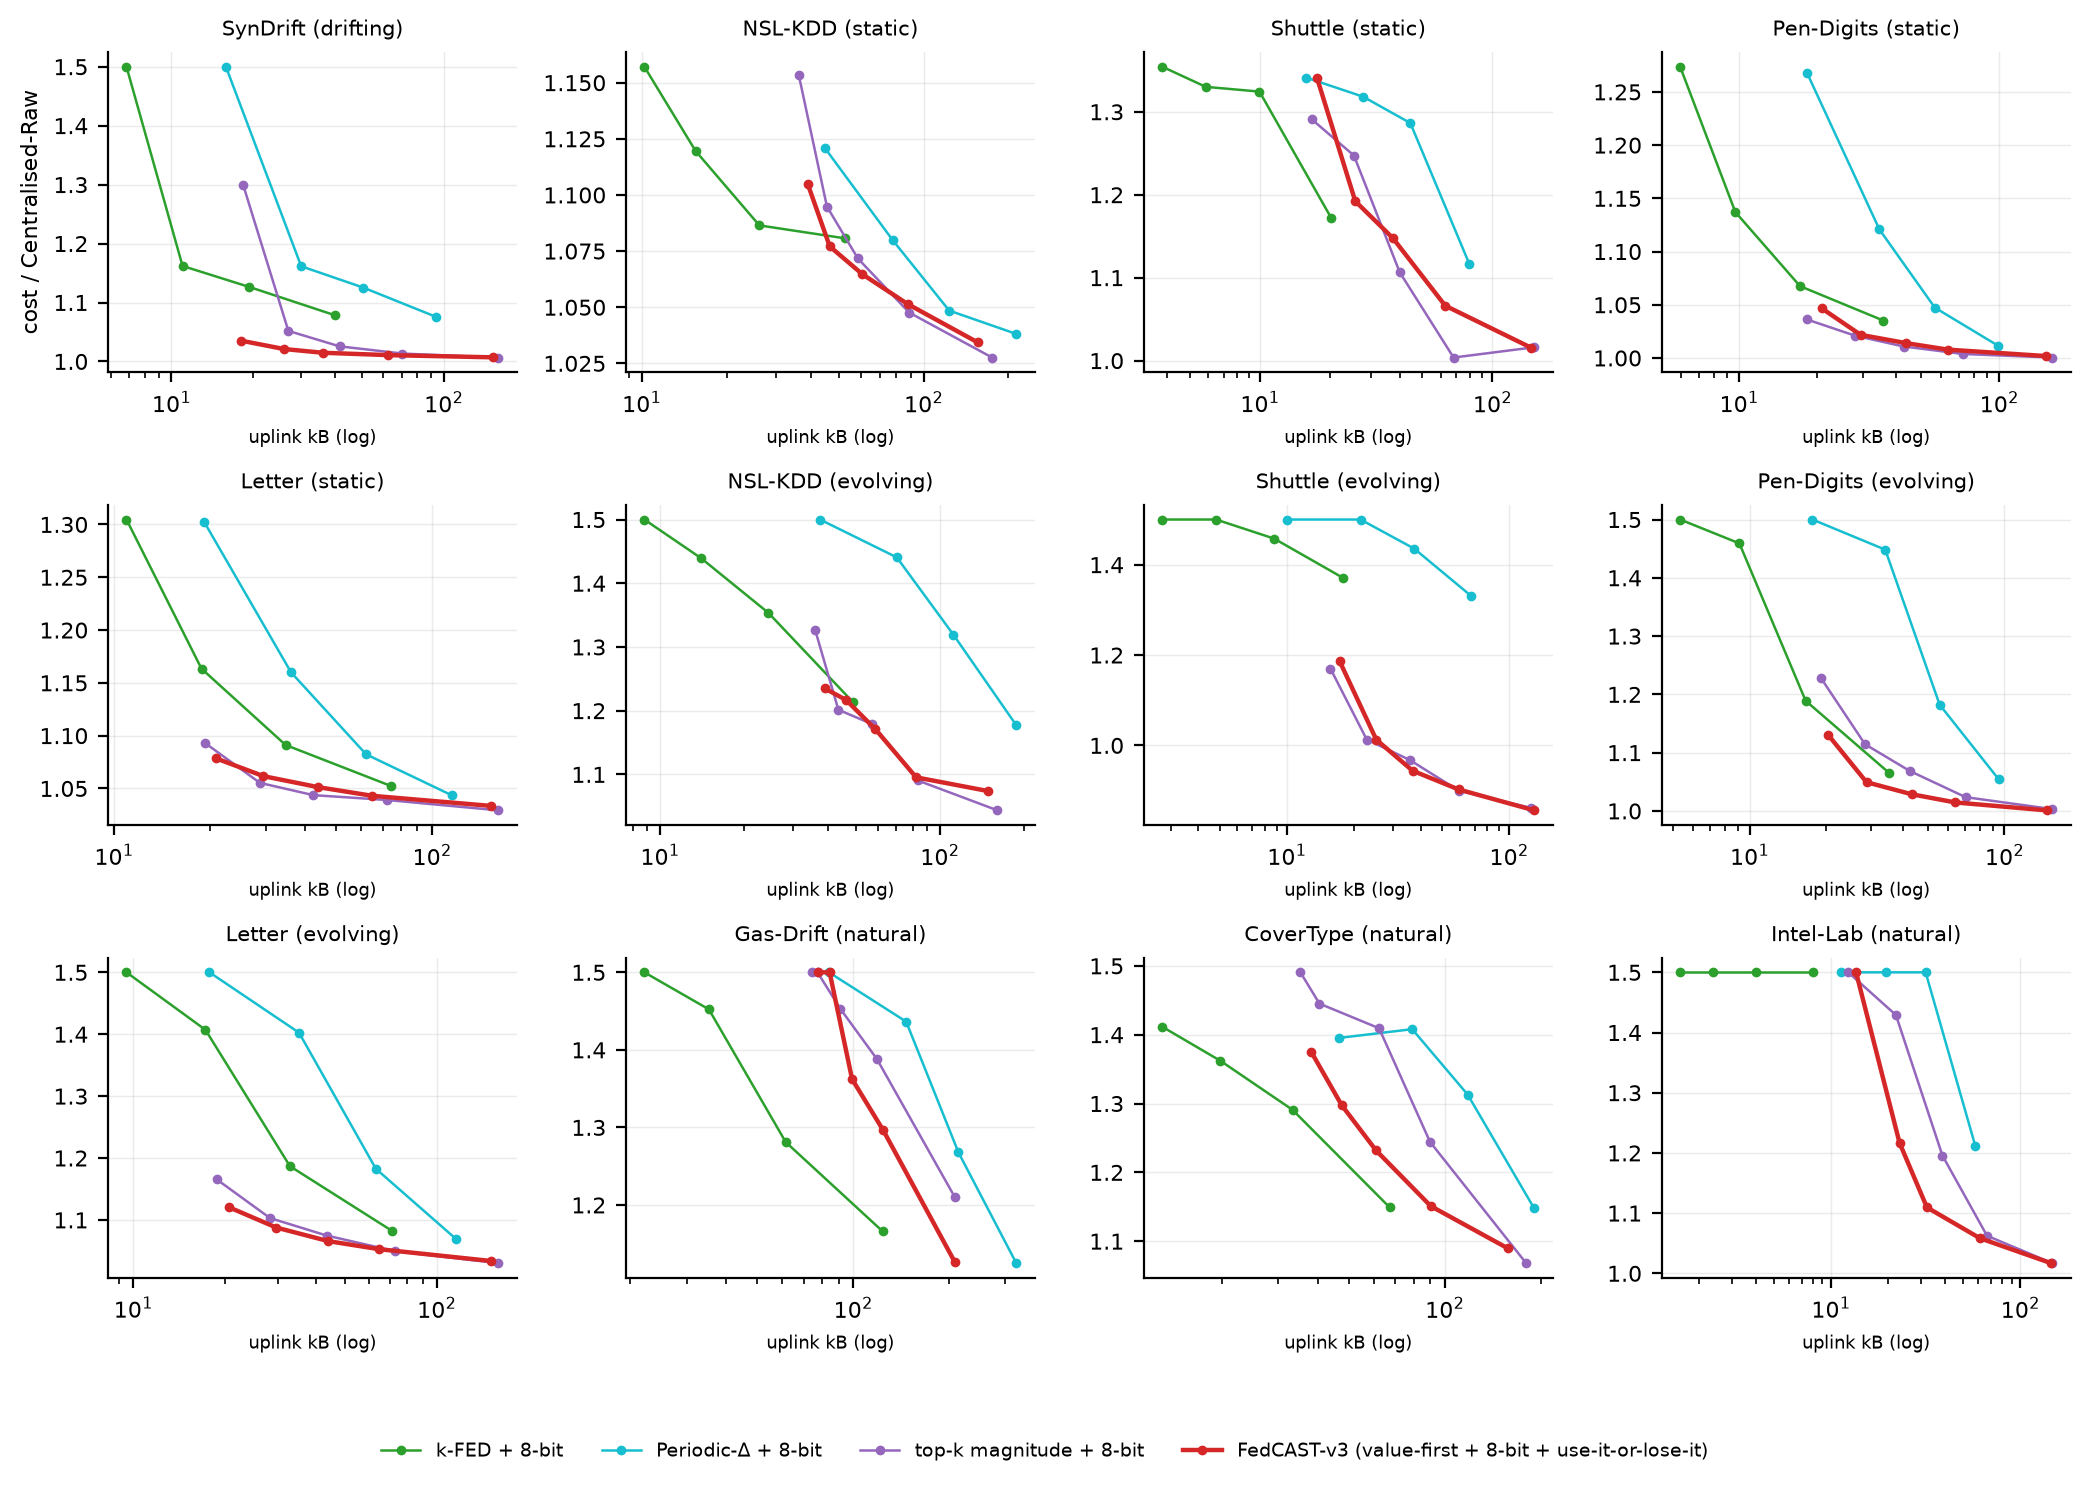
\includegraphics[width=\textwidth]{fig_v3.png}
\caption{Cost ratio vs.\ uplink bytes on twelve settings (mean of 5 seeds; all methods 8-bit). Lower-left is better. Red: FedCAST-v3; purple: top-$k$ magnitude with the same budget controller; cyan: Periodic-$\Delta$; green: k-FED.}\label{fig:v3}
\end{figure*}

\begin{figure}[t]
\centering
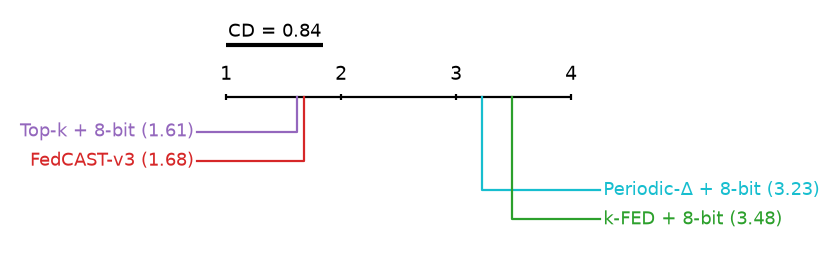
\includegraphics[width=\columnwidth]{fig_cd_v3.png}
\caption{Mean ranks over 31 budget-matched blocks (Nemenyi, $\alpha=0.05$).}\label{fig:cd}
\end{figure}

\subsection{How the Design Evolved (Ablation)}
Table~\ref{tab:evolution} traces the design against the same competitor. Ranking by an objective-linked upper bound (v1) helped only weakly on non-stationary data. The exact value of Proposition~\ref{prop:exact} (v2) made the advantage decisive. Under quantization, v2 plateaued at loose budgets: once all remaining changes had near-zero value it stopped sending, leaving budget unused (NSL-KDD static stayed at 1.043 at 1\,\%, 3\,\% and 10\,\% of raw traffic). The magnitude tie-break and use-it-or-lose-it sends of v3 fixed this and raised the win rate to 72\,\%. 8-bit encoding cut bytes by 2--3$\times$ at equal quality for every method (e.g.\ NSL-KDD evolving reaches 1.10 with 38\,kB instead of 116\,kB). Among the mechanisms shared by all versions, prioritized partial deltas are essential: sending all changed micro-clusters under the same budget raised the cost ratio by up to 32\,\% on SynDrift. Swap search lowered the cost in 17 of 18 non-IID settings (e.g.\ Shuttle 1.107 against 1.218).

\begin{table}[t]
\centering
\caption{Design evolution: win rate against top-$k$ magnitude on non-stationary streams (paired; $p$ one-sided Wilcoxon).}\label{tab:evolution}
\setlength{\tabcolsep}{3pt}
\begin{tabular}{@{}lrrr@{}}
\toprule
Ranking (encoding) & pairs & win & $p$\\
\midrule
v1: objective-linked upper bound (float32) & 130 & 62\,\% & $2.8\times10^{-3}$\\
v2: exact value, Eq.~\eqref{eq:marginal} (float32) & 130 & 75\,\% & $7.4\times10^{-9}$\\
v2: exact value (8-bit, both methods) & 200 & 64\,\% & $1.6\times10^{-7}$\\
v3: + tie-break + use-it-or-lose-it (8-bit) & 200 & \textbf{72\,\%} & $\mathbf{3.9\times10^{-11}}$\\
\bottomrule
\end{tabular}
\end{table}

\subsection{Heterogeneity and Drift}
With the objective-linked policy and the same aggregator, cost ratios stayed at 1.008--1.065 from IID to one-class-per-node partitions on SynDrift, Pen-Digits and Letter, against 1.047--1.126 for periodic sending and 1.067--1.281 for k-FED. Node balancing ($N_i^{0.5}$) helped in the cluster-exclusive regime (Pen-Digits: 1.011 against 1.029). In that regime k-FED with the oracle $k'$ reached higher label agreement (ARI 0.66) at a much higher k-means cost (1.22). On SynDrift, the value-driven trigger reported emerging clusters in 9--11\,s, against 27\,s for periodic updates and k-FED, while sending less (59--87\,kB against 127\,kB). Fig.~\ref{fig:drift} shows the time course, and Fig.~\ref{fig:budget} shows that every node stays within the hard budget envelope.

\begin{figure*}[t]
\centering
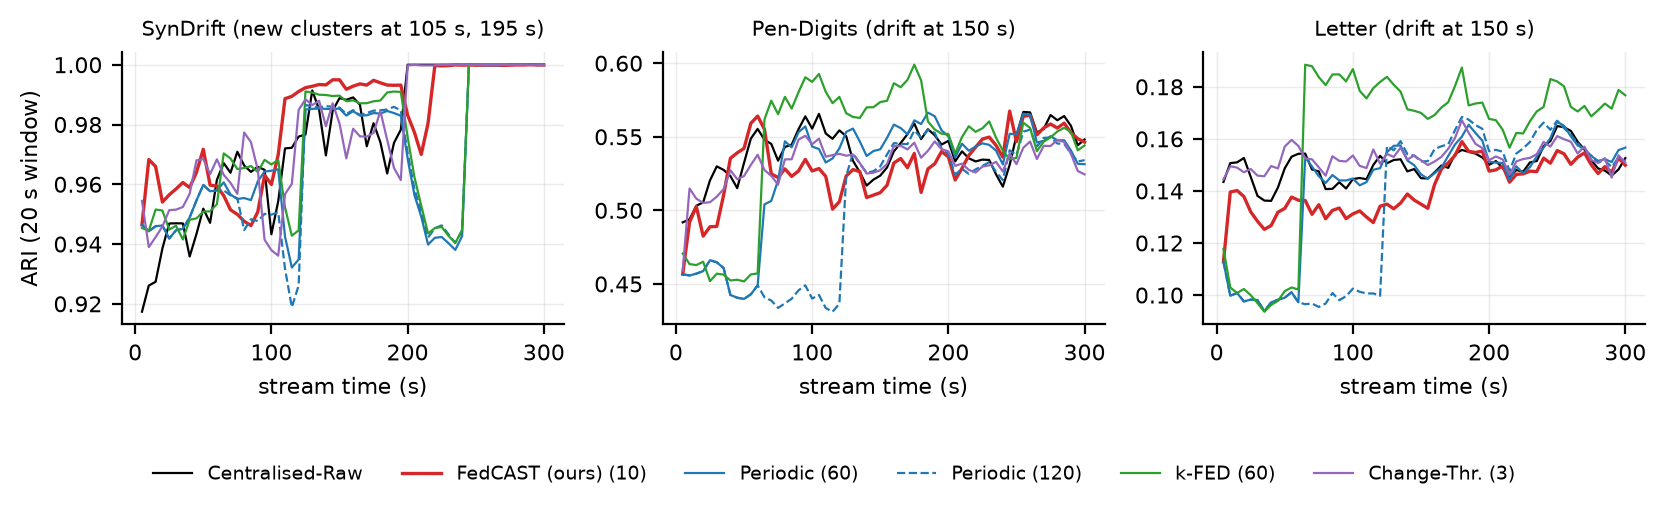
\includegraphics[width=\textwidth]{fig_drift.png}
\caption{ARI over time (20\,s window; mean of 5 seeds). On SynDrift, new clusters emerge at 105\,s and 195\,s; on Pen-Digits and Letter, node class sets rotate at 150\,s.}\label{fig:drift}
\end{figure*}

\begin{figure}[t]
\centering
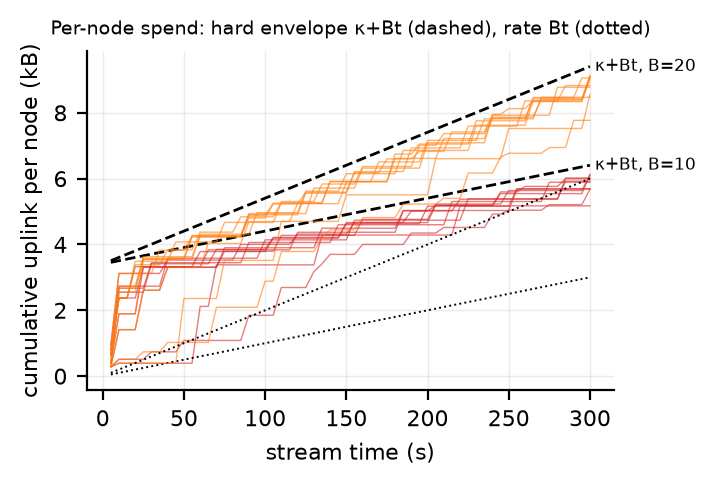
\includegraphics[width=0.9\columnwidth]{fig_budget.png}
\caption{Per-node cumulative uplink with $B/W=10$ and $20$\,B/s. Dashed: hard envelope $\kappa+Bt$ (Proposition~\ref{prop:budget}); dotted: rate $Bt$.}\label{fig:budget}
\end{figure}

\subsection{Systems Evaluation}\label{sec:systems}
\textit{Fault tolerance (real broker).} We killed the coordinator with SIGKILL after 15\,s and restarted it 8\,s later. It restored all node states from the compacted changelog in 1.08\,s, caught up within 0.5\,s, and ended in a state \emph{identical} to that of a shadow coordinator that never failed: the same micro-cluster identifiers and a mass difference of 0.0. All 238 summaries were applied exactly once. When we stopped the broker for 34\,s in the middle of a run, all 231 summaries were delivered and applied, with no loss and no delivery errors.

\textit{Scalability.} From 5 to 50 nodes on one 4-core machine (Fig.~\ref{fig:kscale}), end-to-end latency stayed at 33--35\,ms (p50) and 57\,ms (p95), against 156--179\,ms (p50) for streaming raw data, which shipped 2.5--2.8\,MB against FedCAST's 32--325\,kB. The complete system at 50 nodes used 788\,MB of RAM.

\begin{figure}[t]
\centering
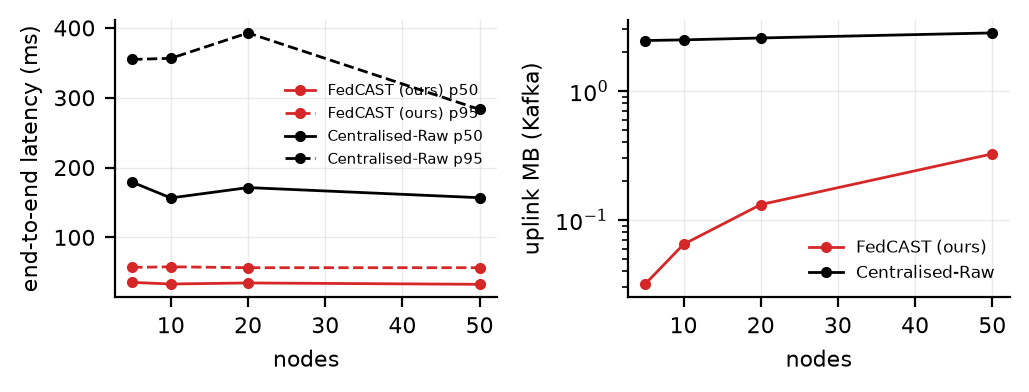
\includegraphics[width=\columnwidth]{fig_kafka_scale.png}
\caption{Real Kafka, 5--50 nodes: end-to-end latency (left) and uplink bytes (right, log scale).}\label{fig:kscale}
\end{figure}

\textit{Multi-container deployment.} Each of 10 edge nodes ran in its own container, with its own network stack and real TCP, against a real broker. Kernel-enforced bandwidth caps (\texttt{tc tbf}: 100\,Mbit, 5\,Mbit, 1\,Mbit and 128\,kbit, round-robin) were applied per node. Quality was evaluated offline from the coordinator's logged models against the simulated centralized learner. Table~\ref{tab:deploy} confirms the simulation results end to end. On the naturally partitioned Intel Lab stream, FedCAST-v3 reached 1.091 with 35\,kB, against 1.188 with 38\,kB for top-$k$ and 2.547 for Periodic-$\Delta$. Every summary was applied, median latency was 31--39\,ms, and each edge container used about 110\,MB.

\begin{table}[t]
\centering
\caption{Multi-container deployment (single runs; 10 edge containers with kernel bandwidth caps; real broker; all methods 8-bit). Uplink kB and cost ratio.}\label{tab:deploy}
\setlength{\tabcolsep}{4pt}
\begin{tabular}{@{}lccc@{}}
\toprule
Stream & FedCAST-v3 & Top-$k$ & Periodic-$\Delta$\\
\midrule
SynDrift & \textbf{35.9 / 1.006} & 40.5 / 1.019 & 30.1 / 1.154\\
Intel Lab (natural) & \textbf{35.4 / 1.091} & 37.9 / 1.188 & 19.6 / 2.547\\
\bottomrule
\end{tabular}
\end{table}

\subsection{What Did Not Work}
We report negative results so that others need not repeat them. (i) A normalized 1:1 blend of an objective bound and magnitude looked excellent in a 3-seed pilot but was ranked \emph{worst} in the full 250-block test. (ii) A novelty override for emerging mass was redundant with the value criterion: detection delays were identical with and without it. (iii) Link-price awareness shifted only 4--7\,\% of traffic away from poor links, and only under loose budgets. (iv) Compressed multi-resolution full summaries (k-FED-style coarsening driven by our trigger) were worse than both k-FED and FedCAST. (v) Data-driven adaptive resolution slid along the existing trade-off curve instead of improving it. (vi) The model-free score $U$ of Theorem~\ref{thm:robust} gives a guarantee but ranks worse than the exact value ($p=5\times10^{-4}$).

\section{Discussion and Limitations}\label{sec:discussion}
\textit{When to use what.} For evolving streams under a byte budget, communicating by value is the right choice. For static streams, top-$k$ magnitude with error feedback is equally good. Both should replace periodic synchronization and one-shot federated clustering, which lose on every non-stationary setting in our evaluation. For well-separated, nearly static local clusters at extremely low byte counts, k-FED remains competitive.

\textit{Kafka as part of the algorithm.} Building the protocol on Kafka's ordering, idempotence, replay and compaction removed whole classes of failure handling from the algorithm, at the cost of a broker that needs about 400\,MB.

\textit{Limitations.} (i) Proposition~\ref{prop:exact} assumes fixed assignments, and the marginal value ignores cross terms with other nodes' unsent changes. (ii) The sandbox kernel lacked \texttt{netem}, so delay and loss were emulated in the application; kernel shaping covered bandwidth only, and deployment results are single runs. (iii) $k$ is assumed known; an unknown-$k$ aggregator~\cite{zhang2025afcl} could replace ours without changing the send policy. (iv) CFs are aggregates but not differentially private. Gaussian noise on the quantized deltas~\cite{epasto2023dpstream} would add a bytes--accuracy--privacy trade-off that the budget controller can also bound. (v) Streams are replayed at an accelerated rate; energy was not measured.

\section{Conclusion}
The value of an update to a federated clustering has an exact closed form, and it is computable on the device. FedCAST uses it to decide what and when to send under a hard byte budget, on top of Apache Kafka with exactly-once state. On non-stationary streams, and most strongly on naturally drifting real data, communicating by value significantly outperforms communicating by magnitude, the federated-learning standard, as well as schedule-based federated clustering, while matching them on static streams. Future work includes an unknown-$k$ aggregator, differential privacy for quantized deltas, a regret analysis of value-greedy sending, and deployments on physical devices over real wireless links.

\bibliographystyle{IEEEtran}
\bibliography{references}

\end{document}
